\documentclass[journal]{IEEEtran}
\usepackage{blindtext}
\usepackage{graphicx}
\usepackage{amsmath}
\usepackage{graphicx}%
\usepackage{url}%
\usepackage{abstract}%
\usepackage{csquotes}
\usepackage{amsthm}
\usepackage{amssymb}

\hyphenation{op-tical net-works semi-conduc-tor}

\usepackage[backend=biber]{biblatex}%
\bibliography{biblio}% The name of your .bib file


\begin{document}
%
% paper title
% can use linebreaks \\ within to get better formatting as desired
\title{Damage localization based on vibrations}


\author{Benjamin Fasquelle, Nicolas Pompidor and Jimmy Rogala}



% The paper headers
%\markboth{Project}{}


% make the title area
\maketitle


\begin{abstract}
abstract
\end{abstract}

\begin{IEEEkeywords}
Damage, Localization, Vibration, Health monitoring
\end{IEEEkeywords}


\IEEEpeerreviewmaketitle



\section{Introduction}

There are four levels for damage identification:
\begin{itemize}
\item detection: Is the structure damaged or not?
\item localization: Where is the damaged area located?
\item quantification: What is the extent of damage?
\item prediction: What is the remaining service life of the structure?
\end{itemize}

\section{State of the art}


\section{Models of vibrating structures}% or Physical models

\subsection{Finite element model}

The dynamic behaviour of a mechanical system consisting of $n$ masses connected
through springs and dampers is described by following matrix differential equation:
\begin{equation}
M \ddot{q}(t) + C \dot{q}(t) + K q(t) = f(t)
\label{fondamental}
\end{equation}
where $q(t)$ is the displacement vector at a continous time $t$, and $M, C, K \in \mathbb{R}^{n \times n}$, are the mass, damping and stiffness matrices. 

For civil engineering structures, Equation (\ref{fondamental}) is obtained as the finite element approximation of the system with only $n$ dregrees of freedom.
The structure is divided in elements, and the global mass matrix $M$ and stiffness matrix $K$ are generated from the geometry and material
properties of the elements.
Due to the lack of identifiable or measurable material
constants that govern the global damping behaviour of a structure, it is generally
impossible to assemble the damping matrix C in the same way as M and K.


\subsection{Continous-time state-space model} %(model parameters and reduction):

From the Equation (\ref{fondamental}) and with the variable change $x =
\begin{pmatrix}
\dot{q} \\
q
\end{pmatrix}$, we obtain the state equation:
\begin{equation}
\dot{x}(t) = A_cx(t) + B_cf(t)
\end{equation}
 where
$A_c =
\begin{pmatrix}
0 & I \\
M^{-1}K & M^{-1}C
\end{pmatrix}$
and
$B_c=
\begin{pmatrix}
0 \\
M^{-1}
\end{pmatrix}$

In a practical vibration experiment, not all $n$ degrees of freedom of the structure are measured, but only
a subset. The observation equation is:
\begin{equation}
y(t) = C_cx(t) + D_cf(t)
\end{equation}

If it is assumed that all $n$ degrees of freedom are measured and that the sensors are accelerometers transducers, we have
$C_c =
\begin{pmatrix}
M^{-1}K & M^{-1}C
\end{pmatrix}$
and
$D_c=
\begin{pmatrix}
M^{-1}
\end{pmatrix}$

Thus, the classical continuous-time state-space model is:
\begin{equation}
\left\{
\begin{array}{ll}
\dot{x}(t) = A_cx(t) + B_cf(t) \\
y(t) = C_cx(t) + D_cf(t)
\end{array}
\right.
\end{equation}

\subsection{Discrete-time state-space model} %(impulses response)

Up to now all equations were expressed in continuous time, whereas in reality
measurements are taken at discrete time instants.
So this model need to be converted to discrete time.
Another reason is that it is needed for performing simulations.

Thus, we choose a certain fixed sampling period $\Delta t$, and the continuous-time equations are discretized and solved at all
discrete time instants $k$ with $t = k \Delta t, k \in \mathbb{N}$.

The discret-time state-space model is:
\begin{equation}
\left\{
\begin{array}{ll}
x_{k+1} & = Ax_k + Bf_k \\
y_k & = Cx_k + Bf_k
\end{array}
\right.
\end{equation}
where
\begin{equation}
\begin{array}{ll}
A = exp(A_c \Delta t) \\
B= (A - I) A^{-1}_c B_c \\
C = C_c \\
D = D_c
\end{array}
\end{equation}



%Stockastic state-space models
%ARMA models
%Continuous time frequency-domain models
%Discrete time frequency-domain models


\section{Localization using FRF interpolation method}

This method is presented in \cite{dilena2015damage}.
The main hypothesis underlying the method is that a concentrated damage reflects in a loss of spatial regularity of the
vibrational profile of a structure, compared with the reference (undamaged) state.

In this section, we suppose that we have $n$ sensors, which are located along an axis $z$, and we denote them by
$\{z_l\}, l\in \{1 ... n\}$. We also suppose we have $N$ measures for each sensor.

For each sensor, we calculate the Frequency Response Function (FRF) from the acceleration's measures, at certain frequencies 
(which are $\frac{k}{N}, k \in \{0 ... N-1\}$).

Thus, for each frequency and each sensor, we have the transfer function value. Let us denote $H_R(z_l,f_i)$ the value of the transfer function for  the sensor $z_l$ at the frequency $f_i$.

Then, we calculate for each sensor $z_l$ the cubic polynomial spline interpolation of the transfer functions $H_R(z_k,f_i)$ measured at all 
the other instrumented locations $\{z_k\}, k\in \{1 ... n\}, k \neq l$: we denote it $H_S(z_l,f_i)$.

For these two transfer functions, we define the interpolation error $E(z_l,f_i)$ as the absolute value of the difference between recorded and interpolated FRFs:
\begin{equation}
E(z_l,f_i) = | H_R(z_l,f_i) - H_S(z_l,f_i) |
\end{equation}


\begin{figure}
  \centering
  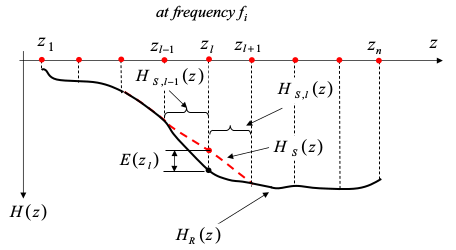
\includegraphics[width=0.4\textwidth]{images/interpolation.png}
  \caption{Interpolation error, from \cite{dilena2015damage}}
  \label{interpolation_error}
\end{figure}


Since we want to characterize each location $z_l$ with a scalar-valued error index, we introduce the norm of the error on the whole range of
frequencies:
\begin{equation}
E(z_l) = \sqrt{  \sum\limits_{i=1}^N  E^2(z_l,f_i) }
\label{error}
\end{equation}


Transfer function values obviously depend on the state of the structure. Hence, if the estimation of the error function
through Equation (\ref{error}) is repeated in the baseline (undamaged) and in the inspection (possibly damaged) configuration, then the
difference between the two values, denoted respectively by $E_0(z_l)$ and $E_d(z_l)$, can provide an indication about the existence of
degradation at location $z_l$:
\begin{equation}
\Delta E(z_l) = E_d(z_l) - E_0(z_l)
\end{equation}

An increase in the interpolation error between the reference configuration and the current configuration at a station $z_l$ , i.e.
$ \Delta E(z_l) > 0$, highlights a localized reduction of smoothness in the vibrational amplitude profile and, therefore, it is assumed
to be a symptom of a local variation of stiffness at $z_l$ associated with the occurrence of damage.

The above analysis has been developed in a deterministic context. Several sources, such as temperature, nonlinear
behavior, soil structure interaction and noise in recorded data, can induce variations of the interpolation error even if no
damage occurs.

Thus, once have to determine a threshold $E_T$, such as $ \Delta E(z_l)$ must be taller than $E_T$ to have a high probability of identification of a damage at location $z_l$. Indeed, as we can see in the Figure (\ref{proba}), the curves which represent the fact to have a damage or not have a share area: if the interpolation error $ \Delta E(z_l)$ is in this area, one can commit two errors:
\begin{itemize}
\item if it is in the area $P_f(z_l)$ under the graph of $p_{E,0}(z_l)$, once can detect a damage since there isn't one (false alarm).
\item if it is in the area $P_m(z_l)$ under the graph of $p_{E,d}(z_l)$, once can not detect a damage since there is one (missing alarm).
\end{itemize}


\begin{figure}
  \centering
  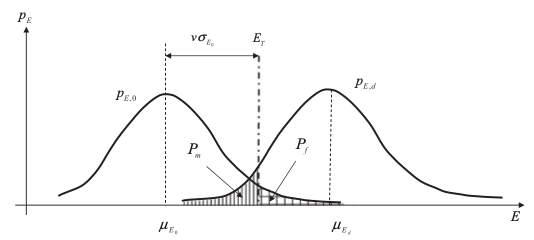
\includegraphics[width=0.4\textwidth]{images/gaussiennes.png}
  \caption{Probabilities of false and missing alarm, from \cite{dilena2015damage}}
  \label{proba}
\end{figure}

\section{Simulation}

%Thus, we consider that we are in the case of Rayleigh damping: the damping 
%matrix is a linear combination of the mass and stiffness matrix:

\section{Conclusion}




%\appendices
%\section{One appendix}
%some text for the appendix.

% use section* for acknowledgement
%\section*{Acknowledgment}
%The authors would like to thank...


%\begin{thebibliography}{1}
%
%\bibitem{IEEEhowto:kopka}
%H.~Kopka and P.~W. Daly, \emph{A Guide to \LaTeX}, 3rd~ed.\hskip 1em plus
%  0.5em minus 0.4em\relax Harlow, England: Addison-Wesley, 1999.
%
%\end{thebibliography}

\nocite{*}
\printbibliography

\end{document}



